\documentclass{article}
\usepackage[utf8]{inputenc}
\usepackage[portuguese]{babel}
\usepackage{enumitem}
\usepackage{a4wide}
\usepackage[a4paper, margin=1in]{geometry}
\usepackage{graphicx}
\usepackage{xcolor}
\usepackage{url}
\usepackage{hyperref}
\usepackage[parfill]{parskip}
\usepackage{fancyhdr}

\def\BibTeX{{\rm B\kern-.05em{\sc i\kern-.025em b}\kern-.08em
    T\kern-.1667em\lower.7ex\hbox{E}\kern-.125emX}}
    
\pagestyle{fancy}
\fancyhf{}

\renewcommand{\headrulewidth}{0.03cm}% 2pt header rule
\renewcommand{\headrule}{\hbox to\headwidth{%
  \color{castanho-ue}\leaders\hrule height \headrulewidth\hfill}}
  
\renewcommand{\footrulewidth}{0.03cm}% 2pt header rule
\renewcommand{\footrule}{\hbox to\headwidth{%
  \color{castanho-ue}\leaders\hrule height \headrulewidth\hfill}}
  
\rfoot{\thepage}

\definecolor{castanho-ue}{HTML}{ad4758}

\pagenumbering{roman}
\begin{document}

\begin{titlepage}

\begin{minipage}{0.7\textwidth}
\noindent\LARGE\textbf{Front-end Developer\\\\}
\Large{Licenciatura em Eng. Informática\\}
\large{Estágio-Projeto 2021-2022\\}
\end{minipage}
\begin{minipage}[t]{0.3\textwidth}\raggedleft

\includegraphics[width=.9\linewidth]{images/di.pdf}
\end{minipage}
\noindent
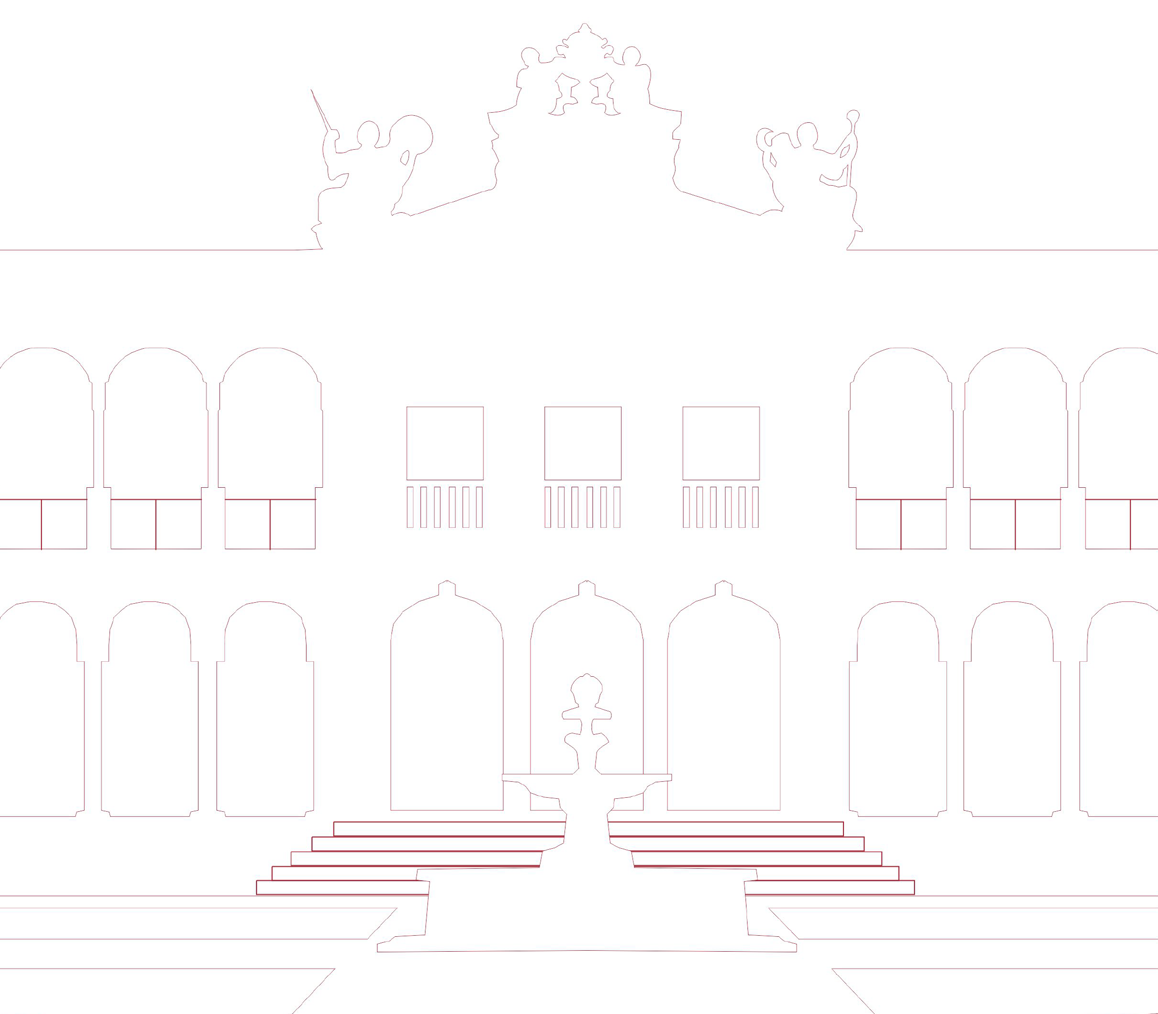
\includegraphics[trim={0 2cm 0 0}, clip,  width=\linewidth]{images/claustros.png}\\

\vspace{0.5cm}
\noindent\textcolor{castanho-ue}{\rule{\textwidth}{0.03cm}}

\vspace{0.5cm}
\noindent\large\textbf{Ricardo Marques Oliveira\\}

\noindent
Orientador na empresa: Fábio Belga\\     
Orientador no departamento: Professor José Saias

\emph{\\Trabalho desenvolvido na empresa Optiply no âmbito da disciplina de Estágio-Projeto da Licenciatura em Eng. Informática.}\\ 

\begin{flushright}
\emph{Évora, \today}
\end{flushright}

\end{titlepage}


\cleardoublepage
\tableofcontents

\cleardoublepage
\pagenumbering{arabic}
\section{Introdução}
\hspace*{0.5cm} Este relatório foi elaborado no âmbito da licenciatura em Engenharia Informática, pertencente ao Departamento de Informática da Escola de Ciências e Tecnologia da Universidade de Évora, pela Unidade Curricular Estágio-Projeto, desempenhado na empresa Optiply. Tem como objetivo a apresentação e descrição de toda a atividade desempenhada, bem como das tecnologias e métodos aplicados no decorrer do estágio. \newline
\hspace*{0.5cm} A educação em contexto laboral, recentemente adotada para a licenciatura em Engenharia Informática, prepara os alunos e proporciona a experiência prática dos conceitos adquiridos no decorrer da formatura, em contexto real no mercado de trabalho propriamente dito. Promove assim, o desenvolvimento de competências, tanto técnicas como organizacionais, cruciais para o futuro. \newline
\hspace*{0.5cm} Em simultâneo, para a instituição que alberga os formandos também retira proveito, uma vez que, facilita os processos de recrutamento de novo pessoal, proporcionando assim também uma constante adaptação à evolução tão constante que existe na área da tecnologia. \newline
\hspace*{0.5cm} O estágio promoveu também, para auxílio mais ativo ao aluno, um orientador na empresa e um orientador no departamento.

\hspace*{0.5cm} As ferramentas utilizadas e mais presentes no decorrer deste período foram \emph{Angular} \cite{angular, angular-wiki, angular-docs, angular-repo} e por consequente, \emph{TypeScript} \cite{ts, ts-docs}, uma vez que \emph{Angular} é baseado nesta linguagem de programação; bem como, uma vez que o projeto baseava-se no desenvolvimento \emph{front-end} \cite{frontend}, \emph{HTML} \cite{html-article, html-wiki} e \emph{CSS} \cite{css}. \newline
\hspace*{0.5cm} Como ferramenta essencial, \emph{Angular}, esta plataforma foi desenvolvida pela \emph{Google} \cite{google} originalmente designada por \emph{AngularJS} \cite{old-angular} (para as versões 1.X da \emph{framework}), foi reescrita pela mesma equipa inicial, estando esta atualmente na versão \textbf{14.0.0}. \newline

\subsection{Enquadramento}
\hspace*{0.5cm} O estágio foi realizado no âmbito da Unidade Curricular Estágio-Projeto da licenciatura em Engenharia Informática da Universidade de Évora, como já foi mencionado, para a empresa Optiply. Empresa esta que é Holandesa, no entanto está sediada também em Portugal, na cidade de Évora. \newline 
\hspace*{0.5cm} Este foi realizado em regime misto, isto é, existiu a flexibilidade e autogestão no tipo de regime que pretendíamos optar. Ou seja, tanto poderíamos realizar uma semana presencialmente nos escritórios da sede da empresa, como realizar as tarefas remotamente. \newline
\hspace*{0.5cm} O mesmo teve duração de 240 horas, tendo início em fevereiro e término no final do mês de maio, sendo que foram realizadas 8 horas diárias, 2 vezes por semana, somando assim 16 horas semanais, ao longo de 15 semanas. Concretamente, teve início a 14 de fevereiro do corrente ano e término a 25 de maio do mesmo ano, concluindo assim a totalidade de horas determinadas. \newline

\subsection{Objetivos}
\hspace{0.5cm} De modo a demonstrar total perceção do que foi realizado no decorrer do estágio, nesta secção serão apresentados os objetivos, de forma integral, propriamente ditos.
\begin{itemize}
  \item Inicialmente, de modo a agilizar a aprendizagem da nova ferramenta \emph{Angular}, a empresa dispôs-nos um curso de introdução à \emph{framework}, através da plataforma de cursos \emph{Udemy} \cite{udemy}, com a duração de mais de 11 horas em aulas com formato de vídeo. Neste curso, a finalidade foi desenvolver 7 projetos distintos para uma perceção das diferentes ferramentas que a \emph{framework} oferece aos seus desenvolvedores;
  \item Após conclusão da etapa anteriormente descrita, iniciou-se a fase seguinte que consistiu na replicação da \emph{Web Application} \cite{webapp} já existente como serviço da empresa;
  \item Finalmente, integrando o último objetivo retratado, finalizou-se o desenvolvimento da mesma aplicação, mas desta vez, em formato \emph{Pair Programming} \cite{pp} em conjunto com o meu colega de curso e neste caso, também de estágio.
\end{itemize}

\vspace*{0.125cm}

\subsection{Contribuições}
\label{sec:cont}
\hspace*{0.5cm} Apesar de ter sido desenvolvida a aplicação quase na sua integridade, o seu caráter foi exclusivamente instrutivo para os formandos, uma vez que o serviço já foi desenvolvido por profissionais da empresa e continua em constante manutenção e atualização. No entanto, acredito que esta versão desenvolvida por nós pode vir a ser utilizada no futuro como plataforma de teste ou adaptada para outra vertente que surja à posteriori. \newline

\subsection{Estrutura do documento}
\hspace*{0.5cm} Após o ponto atual da introdução, seguir-se-á o ponto \hyperref[sec:amb-emp]{Ambiente empresarial}, onde irá ser descrita resumidamente a empresa e também em que envolvente fomos inseridos na mesma.

\hspace*{0.5cm} No \hyperref[sec:est-art]{ponto subsequente} ao último descrito, irão ser mencionadas as soluções propostas ao desafio encarado, bem como as ferramentas ou metodologias que foram adotadas aquando do decorrer das tarefas propostas no estágio.

\hspace*{0.5cm} Após o Estado da arte, prolongar-se-á para o ponto \hyperref[sec:amb-dev]{Ambiente de desenvolvimento}. É neste ponto que serão dadas algumas opiniões pessoais sobre a experiência vivenciada na empresa do ponto de vista de trabalho; é também onde se irão abordar tópicos mais técnicos relacionados com o \emph{hardware} e \emph{software} utilizado; bem como a metodologia de trabalho que a empresa nos proporcionou ou previu que exercêssemos.

\hspace{0.5cm} Segue-se após, a secção do \hyperref[sec:trab-dev]{Trabalho desenvolvido}, no qual será descrito detalhada e pormenorizadamente todo o trabalho realizado durante o período de estágio.

\hspace{0.5cm} Finalmente, previamente às \hyperref[referencias]{Referências} (que será a última página do documento), irá tomar lugar a \hyperref[sec:ava-crt]{Avaliação crítica}, secção final onde serão retratadas as últimas apreciações relativamente ao trabalho realizado.

\cleardoublepage
\section{Ambiente empresarial}
\label{sec:amb-emp}
\hspace*{0.5cm} A Optiply é uma empresa que foi fundada em 2015 em Amesterdão, Holanda por Wiebe Konter; neste momento conta com mais de 50 profissionais, em pelo menos 4 países. A empresa encontra-se numa fase de evolução e esperam começar a operar em mais países da Europa e, se possível, até ao final do ano, ingressar no mercado Asiático. A empresa baseia-se num serviço prestado a terceiros de eficiência de \emph{Supply Chain} \cite{supp-chain}, isto é, uma outra empresa que contrata os serviços da Optiply, poderá ver um aumento no seu volume de negócio, menor \emph{stock} "bloqueado" em armazém e menor tempo desperdiçado em contacto com os fornecedores, uma vez que este serviço automatiza todo o processo e efetua a previsão de vendas para cada produto, delicadamente para cada empresa e cada tipo de mercado em que estas operam. \newline
\hspace*{0.5cm} Os diversos profissionais pertencentes à empresa, operam em distintos setores, tais como, os diferentes ramos das tecnologias de informação, recursos humanos, gestão, consultoria, entre outros. Dos quais tivemos oportunidade de contactar diretamente em contexto profissional. A equipa é constituída na sua grande maioria por novos talentos jovens e proporciona bastantes estágios curriculares nas diversas áreas em que opera, nos diferentes países. \textbf{TODO: EXPLICAR COMO SE "DIVIDEM" AS EQUIPAS NA EMPRESA}\newline
\hspace*{0.5cm} A sede da Optiply em Portugal, como já foi referido, encontra-se na cidade de Évora e é constituída por 3 escritórios modernos e amplos; dos quais podemos contar com salas de reuniões, espaços de trabalho comuns e privados (de modo a permitir melhor comunicação nos trabalhos em equipa, como os que exigem maior concentração e necessitam de mais privacidade) e uma ampla sala comum (designada de \emph{lounge}), onde os funcionários podem fazer uma pausa. A empresa consegue assim, promover um espírito de equipa e cooperação bastante assente, bem como um excelente ambiente entre todos os trabalhadores, não só a nível nacional, mas também com os colaboradores de outros países. O ambiente que se instala nas instalações, é o equilíbrio perfeito entre o formal/informal e profissional/social. Com isto, todos os estagiários que deram entrada, em simultâneo, na empresa no passado mês de fevereiro sentiram-se bastante bem acolhidos e integrados nos seus postos. \newline
\hspace*{0.5cm} A empresa acolheu 4 alunos de 2 instituições distintas, a Universidade de Évora e o Instituto Politécnico de Beja; criando assim a possibilidade de contacto entre pessoas com métodos de formação totalmente distintos, podendo assim abranger alguns conhecimentos e metodologias. Fui integrado na equipa de \emph{Front-end developers}, no entanto, como mencionado nas \hyperref[sec:cont]{Contribuições}, não lidei diretamente com o cliente. Esta mesma equipa, liderada pelo \emph{Development Team Lead} e também Orientador na empresa, Fábio Belga, é constituída na sua totalidade por colaboradores portugueses, com os quais consegui ter contacto direto quando realizei as tarefas em regime presencial. \newline

\cleardoublepage
\section{Estado da arte}
\label{sec:est-art}
Se no âmbito do seu trabalho de estágio fez o levantamento e/ou análise de várias soluções, ferramentas ou metodologias, com o objetivo de escolher a melhor, deve incluir uma descrição desse trabalho nesta secção, incluindo as conclusões a que chegou.
Esta secção pode não fazer sentido em alguns trabalhos.


\cleardoublepage
\section{Ambiente de desenvolvimento}
\label{sec:amb-dev}
\hspace*{0.5cm} Ao iniciar o estágio, realizou-se uma breve reunião de boas-vindas, na qual estiveram presentes, para além dos novos estagiários, o \emph{Development Team Lead} - Fábio Belga e o \emph{Talent Acquisition} - João Fernandes (com o qual realizámos toda a fase de recrutamento). Nesta conferência, foi-nos apresentada novamente a empresa, desta vez de modo mais detalhado, explicado quais seriam as tarefas para ambas as equipas (quer de \emph{Front-end Developers}, como \emph{Back-end Developers}). Nesta etapa foi-nos também atribuído um \emph{e-mail} da empresa, o qual deveríamos começar a utilizar para qualquer situação relacionada com o estágio. \newline

\subsection{Ambiente técnico}
\subsubsection{Hardware}
\hspace*{0.5cm} A empresa não concedeu qualquer tipo de máquina aos alunos que realizaram o estágio, no entanto, sempre que nos deslocámos à empresa, tivemos à disposição todo o tipo de periféricos para proporcionar uma melhor prestação e maior conforto. \newline

\hspace*{0.5cm} Assim sendo, utilizei a minha máquina pessoal para realizar o estágio, sendo ela constituída por um processador \emph{Intel Core i7 9750H}, 16GB de memória, \emph{NVIDIA GeForce RTX 2060} como placa gráfica e 2 discos rígidos, de 512GB SSD NVMe e outro de 1TB SSD M.2. Possui um \emph{dual-boot} com opção entre os 2 Sistemas Operativos que utilizo, sendo eles Linux com distribuição Ubuntu na versão 21.10 e Windows 10 Pro; de realçar que durante todas as tarefas do estágio foi utilizado exclusivamente Ubuntu. \newline

\hspace*{0.5cm} Aos servidores com os quais a empresa atua, não nos foi garantido acesso, uma vez que não seria necessário para a realização de nenhuma tarefa designada durante o decorrer do estágio. \newline

\subsubsection{Software}
\hspace*{0.5cm} Em contexto empresarial/profissional, na área das tecnologias de informação, um \emph{software} essencial na comunicação entre todos os envolventes de uma empresa é o \emph{Slack} \cite{slack}, plataforma que nos foi logo apresentada e demonstrada. Através desta, existiu o contacto tanto com membros internos como externos à equipa em que estava incluído. \newline
\hspace*{0.5cm} Para a realização propriamente dita das tarefas atribuídas no decorrer do período do estágio, foram utilizadas diversas ferramentas que são bastante utilizadas atualmente pela maioria das empresas da área, nomeadamente:
\begin{itemize}
    \item \textbf{Angular} - plataforma de desenvolvimento de aplicações \emph{web} e \emph{front-end} utilizada como base para a realização de todas as tarefas; uma vez que é desenvolvida sobre \emph{TypeScript}, este \emph{software} acabou por ser também utilizado. Associado também ao \emph{Angular}, foi utilizada a biblioteca (\emph{Librabry}) da mesma, \emph{Angular Material}. Esta biblioteca contem \emph{user interfaces} por defeito que podem ser utilizadas, de modo a acelerar o processo de desenvolvimento, evitando assim que o desenvolvedor crie constantemente o mesmo tipo de elementos. Foi a primeira vez que tive interação com esta ferramenta, de modo que não foi acessível numa fase inicial, porém, com o decorrer das atividades, habituei-me rapidamente.
    \item \textbf{TypeScript} - linguagem de programação que teve que ser inevitavelmente utilizada, uma vez que \emph{Angular} é baseado nela. Mesmo sendo a primeira vez que tive contacto com esta linguagem, sendo ela um \emph{superset} de \emph{JavaScript} (linguagem esta com a qual já estava familiarizado, uma vez que foi alvo de estudo em diversas Unidades Curriculares da licenciatura), adaptei-me com bastante facilidade às características da mesma.
    \item \textbf{HTML} - linguagem utilizada de forma consideravelmente reduzida e igualmente, como objeto de estudo em contexto académico, já tinha tido contacto com esta, logo não enfrentei qualquer dificuldade na utilização da mesma.
    \item \textbf{CSS} - este mecanismo de estilização é aplicado diretamente num documento \emph{web}, à semelhança de \emph{HTML}, também já tinha tido contacto com esta ferramenta, no entanto adquiri novos conceitos da mesma.
    \item \textbf{Jira} - ferramenta que permite a monitorização e acompanhamento das tarefas de um projeto em tempo real por parte de uma equipa de trabalho. Ferramenta esta que é bastante utilizada em contexto real de trabalho e a qual nunca tinha tido contacto, no entanto é bastante percetível e de fácil manuseamento.
    \item \textbf{Bitbucket} - sistema de controlo de versões distribuído e hospedeamento de projetos. Ferramenta que, à semelhança do \emph{Jira}, é bastante útil profissionalmente e nunca tinha tido também interação com a mesma.
    \item \textbf{Github} - também é uma plataforma de sistema de controlo de versões, utilizada anteriormente por mim e utilizada nas tarefas feitas de forma singular.
\end{itemize}

\subsubsection{Ambiente aplicacional}
\hspace*{0.5cm} O projeto desenvolvido, no que toca ao seu contexto aplicacional, uma vez que, como já referido, foi criar uma réplica do \emph{front-end} da aplicação do serviço da empresa, considera-se que este é \emph{standalone} não interagindo assim com outros sistemas da empresa; correndo assim, somente localmente na máquina que utilizei no decorrer do estágio. Podemos considerar que a única interação que esta teve, foi com \emph{RESTful APIs} \cite{rest-api} (\emph{Representational State Transfer Application Programming Interface}) de um modo genérico para utilizar dados na criação de elementos do \emph{Angular Material} que fossem preenchidos automaticamente. \newline

\subsection{Metodologia de trabalho}
\hspace*{0.5cm} Num fase inicial do estágio, de modo a uma mais rápida introdução e aprendizagem da \emph{framework Angular}, fomos introduzidos a um curso da mesma, através da plataforma de \emph{e-learning Udemy}. O curso propriamente dito tinha a duração de mais de 11 horas com formato de vídeo, com a finalidade de termos contacto com as principais mecanismos da \emph{framework}, de modo a conseguirmos iniciar o projeto propriamente dito. No entanto, como o curso abrangia um total de 7 pequenos projetos, a duração do mesmo prologou-se para mais horas, devido ao tempo despendido na realização desses mesmos projetos. \newline
\hspace*{0.5cm} Na fase seguinte, quando abordámos o projeto pela primeira vez, foi feito de forma singular, isto é, não foi realizado trabalho em equipa/grupo, logo a gestão e planificação do mesmo foi feita de forma livre por cada um dos formandos. Tomei então a decisão de utilizar o \emph{Github} como controlador de versões e o \emph{Trello} para planificar as minhas tarefas (plataforma idêntica ao \emph{Jira}, mas esta ainda não me tinha sido apresentada). \newline
\hspace*{0.5cm} Na última fase do projeto, trabalhei em equipa, utilizando desta vez o \emph{Jira} com um único \emph{board} dividido em 3 colunas (\emph{TO DO}, \emph{IN PROGRESS} e \emph{DONE}), juntamente com o \emph{Backlog} do mesmo (não utilizando a opção de \emph{sprints} propriamente dita). Assim, adaptou-se um desenvolvimento ágil de \emph{software}, \emph{Pair Programming} mais propriamente dito. \newline
\hspace*{0.5cm} Semanalmente reunimos com o \emph{Development Team Lead} de modo a discutirmos o trabalho que estava a ser realizado, tirar alguma questão mais complicada (que não tivéssemos oportunidade de apresentar aos restantes membros da equipa de \emph{Front-end developers}) e/ou serem apresentadas novas tarefas. \newline

\cleardoublepage
\section{Trabalho desenvolvido}
\label{sec:trab-dev}
\hspace*{0.5cm} Quando iniciei o estágio na Optiply, o \emph{Development Team Lead}, como já foi referido, encaminhou-me a mim e ao meu colega que também iniciou estágio na mesma altura que eu, para um curso na \emph{Udemy} para introdução à \emph{framework Angular}, com aulas em formato de vídeo com duração de mais de 11 horas, contemplando a realização de 7 projetos nos quais começámos a interagir, pela primeira vez, com os blocos principais de desenvolvimento de \emph{Angular}, tais como \emph{components}, \emph{modules}, \emph{services}, \emph{models} e \emph{Angular Material}. No último projeto do curso, o objetivo foi criar um novo projeto que englobasse todos aqueles realizados até então e, deste modo, percebi a facilidade com a qual conseguimos reutilizar código em \emph{Angular}, uma vez que com pequenas alterações conseguimos utilizar as funcionalidades implementadas em outros projetos. Em suma, foi criado um \emph{dashboard} onde, através da seleção num menu implementado nesta fase, escolhemos um projeto anteriormente realizado e, através das \emph{routes} do \emph{Angular}, a \emph{SPA (Single Page Application)}, atualizava com a \emph{component} correspondente. \newline

\hspace*{0.5cm} Após concluir o curso e todos os projetos nele englobados, ingressei na equipa de \emph{front-end developers} de modo a iniciar o projeto principal do estágio, contudo continuei a trabalhar de forma singular. No entanto, comecei a compreender como toda a equipa trabalhava em conjunto e sempre disponível para me auxiliar nas dúvidas que iam surgindo e a cooperar no meu raciocínio para a resolução dos obstáculos que foram aparecendo. Esta foi a fase do estágio que tomou a maior parte do tempo, uma vez que o \emph{Angular} apresenta múltiplas funcionalidades e diferentes modos de abordar e resolver cada conteúdo; uma vez que era também a primeira vez que lidava com a \emph{framework} e a nova linguagem \emph{TypeScript}, foram necessárias bastantes horas a ler documentação, pesquisa e de habituação às novas ferramentas. \newline

\hspace*{0.5cm} Na fase final do projeto a desenvolver, foi quando realmente comecei a trabalhar em equipa, juntamente com o meu colega de estágio, na qual continuámos com o desenvolvimento do projeto da fase anterior (a replicação da aplicação \emph{web} já existente da empresa). Utilizando agora o \emph{Jira} e \emph{Bitbucket} de modo a agilizar as funções que teríamos que desempenhar para a conclusão da tarefa. Uma vez que éramos dois formandos sem qualquer tipo de experiência com estas ferramentas totalmente incomuns para nós, senti que foi a fase que foi mais complicada, tanto para conciliar os horários e trabalharmos em conjunto como de compreensão deste tipo de \emph{software}. \newline

\hspace*{0.5cm} Durante a última fase do estágio, a empresa adquiriu um novo espaço de modo a expandir as suas infraestruturas, juntamente à sede já existente, e ao qual fomos convidados para ajudar na logística e preparação do novo espaço. Todos os formandos aceitaram e, juntamente com alguns dos profissionais da empresa, passámos o dia a organizar o material que chegou, bem como na montagem de mobília e disposição da mesma no local. Esta atividade que não estava previamente programada nos conteúdos do estágio foi efetivamente positiva, elevando algumas \emph{soft skills}, nomeadamente o espírito de equipa, flexibilidade e pensamento crítico. \newline

\subsection{Descrição detalhada}
\subsubsection{Curso Udemy}
\hspace*{0.5cm} O curso foi bastante importante, na minha opinião, uma vez que proporcionou-nos uma relevante nota introdutória à nova ferramenta que foi abundantemente utilizada no decorrer do projeto. A escolha do curso, por parte da empresa, pareceu-me bastante acertada, uma vez que, para além das aulas em formato de vídeo, apresentou vários projetos; ou seja, experienciei que, para além de estar a interiorizar os conceitos teoricamente, estar em simultâneo a desenvolver breves projetos, nos quais eram aplicados esses mesmos conceitos teóricos, agilizou e acelerou o processo inicial de aprendizagem (aplica-se tanto para o \emph{Angular} propriamente dito, bem como para a linguagem \emph{TypeScript}).

\subsubsection{Replicação front-end}
\hspace*{0.5cm} Replicar a aplicação \emph{web} do serviço da Optiply foi uma tarefa que, inicialmente necessitou de bastante pesquisa e análise de documentação. No entanto, experienciei que realizar uma réplica, através de imagens da já existente aplicação foi mais acessível do que realizar um projeto totalmente de raiz, sem um guia a seguir. \newline

\hspace*{0.5cm} O desenvolvimento da aplicação, iniciou-se com a elaboração da \emph{toolbar} e do \emph{sidenav}, utilizando \emph{Angular Material}; neste ponto, existiam várias opções viáveis que podiam ser tomadas: gerar um novo \emph{component} para cada um dos \emph{materials}, gerar um novo \emph{component} para ambos os \emph{materials} ou incorporar ambos no \emph{component} da \emph{app} em si. A decisão que tomei, uma vez que ambos estes \emph{materials} seriam \underline{sempre estáticos}, foi desenvolve-los diretamente no \emph{component} principal da aplicação. \newline

\hspace*{0.5cm} De seguida, para a implementação das restantes páginas da aplicação, a melhor decisão a tomar foi criar um \emph{component} para cada uma delas e, assim sendo, foi possível gerar as diversas ferramentas necessárias para cada um deles, nomeadamente \emph{services} (para comunicação com \emph{RESTful APIs}) e \emph{models} (de modo a receber e gerenciar os dados recebidos das \emph{APIs} externas). Nesta tarefa, foi também importante compreender na totalidade, o funcionamento de \emph{routes} em \emph{Angular}, de modo a fazer com que a aplicação fosse totalmente dinâmica e atualizasse a \emph{SPA} consoante a página que fosse solicitada.

\hspace*{0.5cm} Nesta etapa, adquiri os conhecimentos práticos suficientes para o total desenvolvimento de uma aplicação utilizando \emph{Angular}, ferramenta esta que esta a ser cada vez mais presente no mundo profissional.

\cleardoublepage
\section{Avaliação crítica}
\label{sec:ava-crt}
\hspace*{0.5cm} Nesta última secção do relatório do projeto, realizado em regime de estágio curricular, numa empresa que permitiu contacto mais real com a nossa área de estudo, em contexto profissional, resta refletir sobre a minha expectativa inicial perante este novo desafio e transmitir a minha perspetiva global da mesma. \newline

\hspace*{0.5cm} Inicialmente, não aguardava uma fase de recrutamento tão concreta como aquela que nos foi proporcionada, o que me surpreendeu pela positiva, preparando-me assim certamente para o meu futuro profissional e futuras entrevistas. \newline
\hspace*{0.5cm} No que toca à receção por parte de todos os colaboradores da Optiply, também me surpreendeu bastante pela positiva, uma vez que, de imediato me senti totalmente integrado no ambiente da empresa. Obtive rapidamente a perceção de que há o equilíbrio perfeito entre a informalidade e a formalidade. A flexibilidade que foi proporcionada tanto no regime de trabalho (remoto ou presencial) como nos dias semanais nos quais pretendíamos realizar o estágio também foi um aspeto bastante positivo que me motivou ainda mais, desde cedo. \newline

\hspace*{0.5cm} Os pontos menos positivos que tenho a apontar desta etapa foram a realização de um projeto que não esteve diretamente ligado com clientes e com a equipa em que estive integrado, na sua totalidade. Bem como a última fase do projeto em qual tivemos que realizar, em equipa totalmente inexperiente uma colaboração, através do \emph{Jira} e \emph{Bitbucket} para finalizar o projeto, o que não se sucedeu com a maior das facilidades. Outra observação que julgo pertinente de apontar, é o regime ao qual o estágio nos é proposto, isto é, sinto que teria sido muito mais proveitoso para os formandos se este fosse realizado a tempo inteiro, de modo a envolver mais os alunos na realidade empresarial, replicando assim, ainda mais o mundo profissional. \newline
\hspace*{0.5cm} Outro assunto que me causou alguma surpresa, não tão positiva, foi o facto de não termos utilizado qualquer tipo de testes, sendo que desde a fase inicial do projeto, constatei que o \emph{Angular} possui, por defeito, testes já incorporados na \emph{framework}, desde o momento da criação do projeto, até mesmo quando são gerados novos \emph{components}. Sempre tive a noção de que os testes são sempre utilizados abundantemente quando em contexto laboral, logo esperei, à partida, de os empregar num projeto desta importância.

\hspace*{0.5cm} Em suma, refletindo em relação às últimas semanas nas quais desempenhei um papel ativo no projeto de estágio, foram uma mais valia no meu percurso académico de aprendizagem. Evoluindo assim tanto as \emph{soft skills} necessárias ao mercado de trabalho, bem como as \emph{hard skills} da área de estudo e de todas as tecnologias com as quais lidei ativamente. Assim, julgo ter aproveitado bastante o estágio curricular que nos é proporcionado através do Departamento e da Universidade, enriquecendo os conhecimentos adquiridos ao longo de toda a licenciatura.

\cleardoublepage
\bibliographystyle{unsrt}
\bibliography{bibs}
\label{referencias}

\end{document}
